\chapter{反射音方向分布特性}

\section{反射音の方向情報}
反射音の方向情報をみるため、解析で得られたインパルス応答から鉛直方向成分、側方成分、前後方向成分に分解した。なお、反射音の到来角度は音源方向を$0^\circ$とした。
初期反射音($t$=0$\sim$80[ms])の側方成分は観測高さによる違いは見られないものの、鉛直方向成分は座席面遠方音場($H$=14.0)において豊富に到来しているのに対し、座席面近傍音場($H$=1.2)では著しく不足している。

\includepdf[pages=-, angle=90]{05_att/ir_rec3.pdf}

\section{反射音方向別エネルギ比}
ここで、反射音の到来方向バランスを定量的に把握するため、初期反射音の全エネルギ($t$=0$\sim$80[ms])に対する鉛直方向成分の割合$ER_V$(vertical energy ratio)、側方成分の割合$ER_L$(lateral energy ratio)、前後方向成分の割合$ER_G$(longitudinal energy ratio)を各々算出した(\textbf{式}\ref{eq:ERV}$\sim$\ref{eq:ERG})。ここで$\delta$は仰角(鉛直上方向:0$^\circ$)、$\theta$は水平角(側方:0$^\circ$)を表す。

\begin{table}[htbp]
\begin{equation}
  \label{eq:ERV}
  ER_V = {\frac{\displaystyle\int_0^{80}p^2(t)cos^2{\delta}dt}{\displaystyle\int_0^{80}p^2(t)dt}} 
\end{equation}

\begin{equation}
  \label{eq:ERL}
  ER_L = {\frac{\displaystyle\int_0^{80}p^2(t)sin^2{\delta}cos^2{\theta}dt}{\displaystyle\int_0^{80}p^2(t)dt}} 
\end{equation}

\begin{equation}
  \label{eq:ERG}
  ER_G = {\frac{\displaystyle\int_0^{80}p^2(t)sin^2{\delta}sin^2{\theta}dt}{\displaystyle\int_0^{80}p^2(t)dt}} 
\end{equation}

\centering
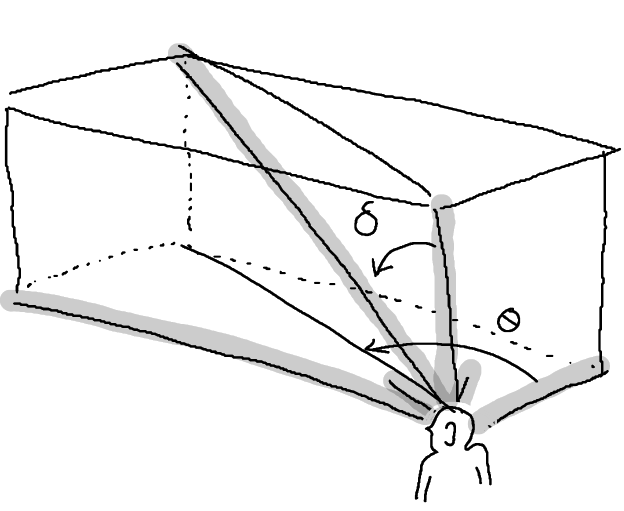
\includegraphics[keepaspectratio,scale=1]{04_att/direction.png}
\label{fig:}
\end{table}

\pagebreak
\section{$DUI$の導入}
ここで鉛直方向・側方・前後方向から反射音エネルギが均等に到来するとき、$ER_V$、$ER_L$、$ER_G$の3値は全て$\frac{1}{3}$となることから、反射音の到来方向に関する空間バランスを見るための指標として3次元直交座標系における点($ER_V$,$ER_L$,$ER_G$)と点($\frac{1}{3}$,$\frac{1}{3}$,$\frac{1}{3}$)の距離$d_i$を観測点ごとに求め(\textbf{式}\ref{eq:di})、その空間内全観測点の平均値として$DUI$(Directional Uniformity Index)$^{\text{\cite{後期音}}}$を算出する(\textbf{式}\ref{eq:DUI})。以後、$DUI$を用いて反射音到来方向分布の一様度の評価を行う。
\begin{table}[htbp]
\begin{equation}
  \label{eq:di}
  d_i = \sqrt{\left({ER_V-\frac{1}{3}}\right)^2 + \left(ER_L-\frac{1}{3}\right)^2 + \left(ER_G-\frac{1}{3}\right)^2} 
\end{equation}
\begin{equation}
    \label{eq:DUI}
    DUI=\frac{\sum_{i=1}^N{d_i}}{N}
\end{equation}
\end{table}

\pagebreak
\section{観測点の座標系について}
反射音方向分布特性をみるにあたり、観測点における座標系の置き方について2通りの検討を行った(\figref{observing})。\\
(i)観測点の座標系を解析モデルの3次元直交座標系にあわせる(正面:y軸負の方向)\\
(ii)観測点の座標系を音源中心の極座標系にする(正面:音源)\\
(i),(ii)それぞれの場合の$ER_V$、$ER_L$、$ER_G$及び$d_i$の分布を観測高さ$H$[m]ごとに示す。

\begin{figure}[htbp]
    \centering
    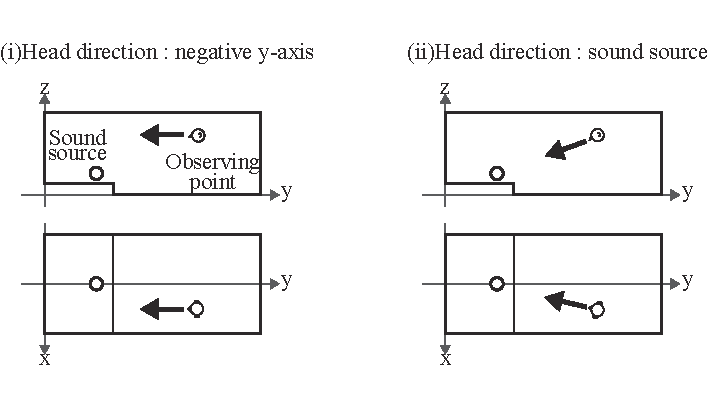
\includegraphics[keepaspectratio,scale=1]{05_att/observing.pdf}
    \caption{\hspace{1mm}\textbf{Study of head direction}}
    \label{fig:observing}
\end{figure}

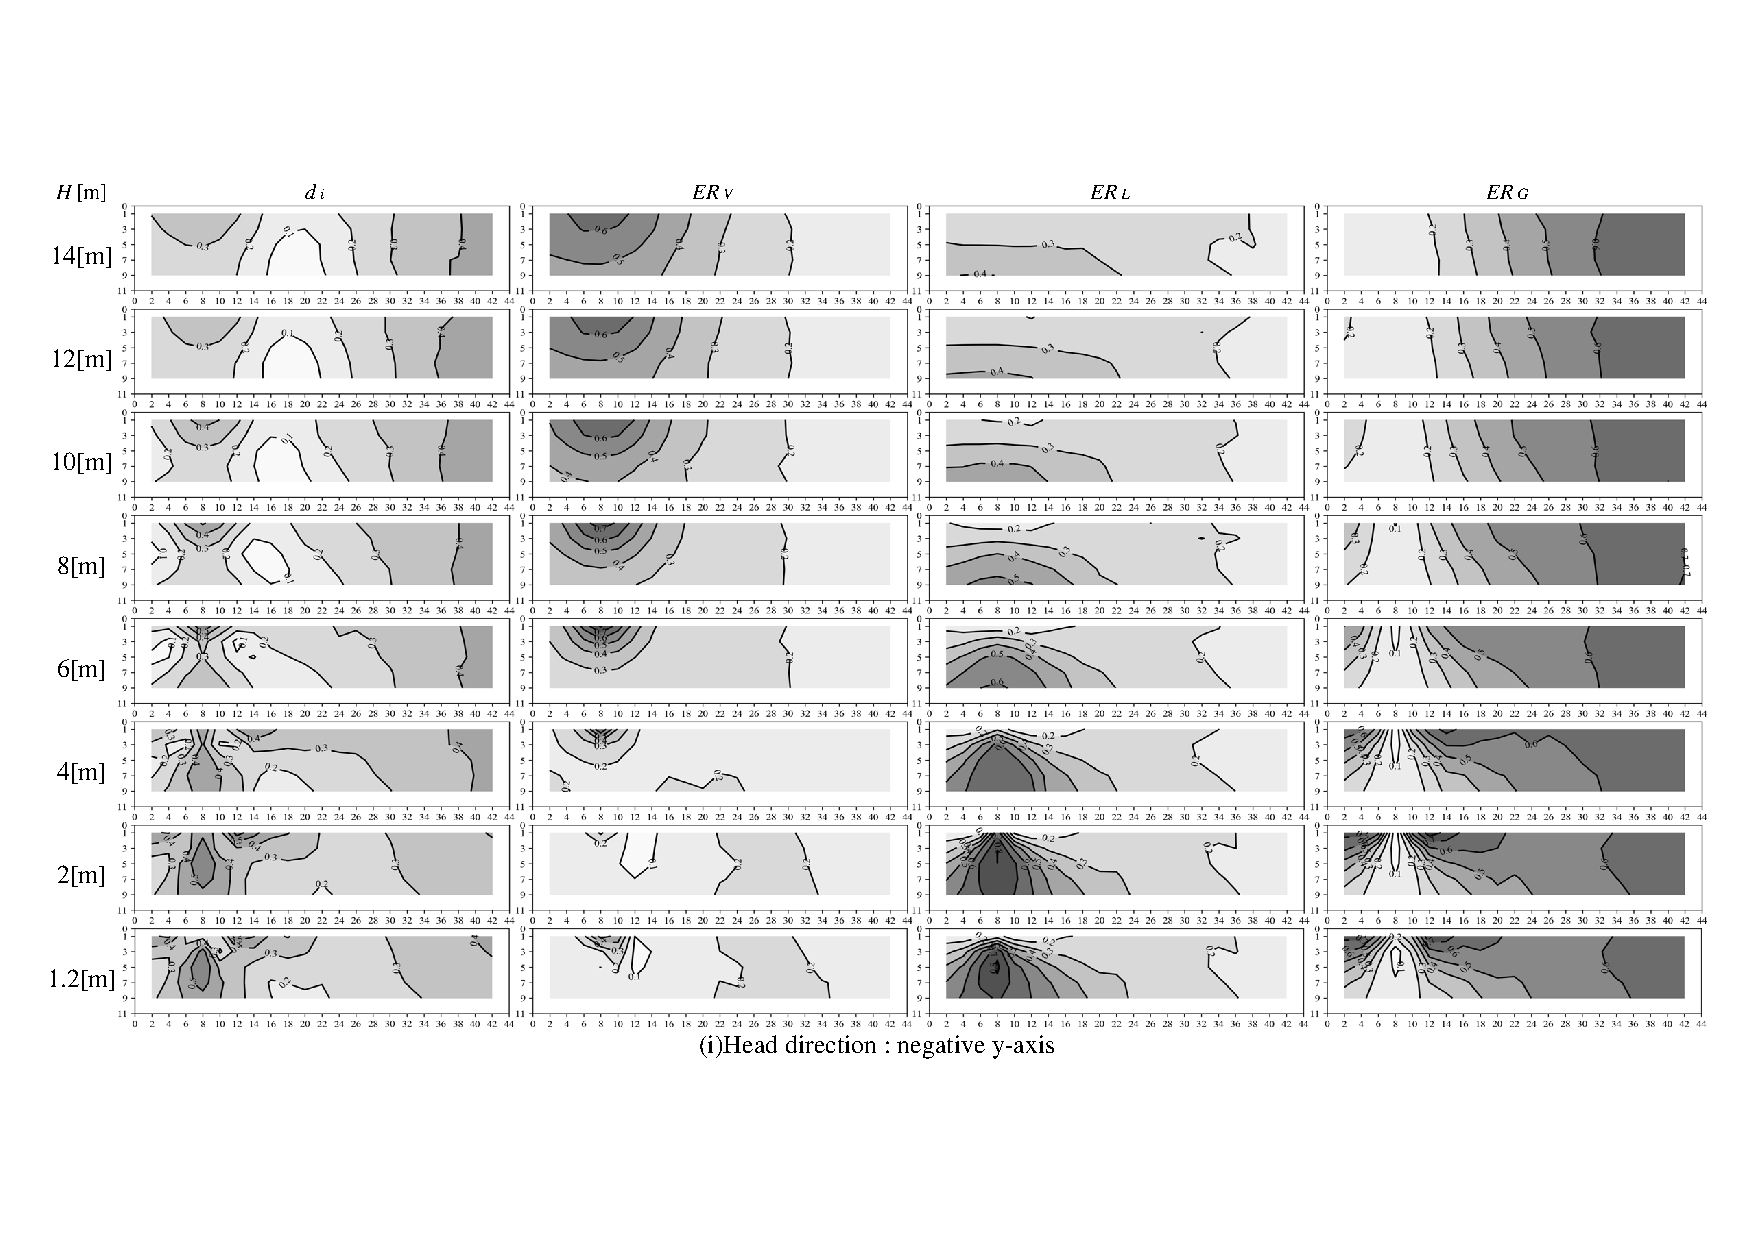
\includepdf[pages=-]{05_att/cont_y.pdf}
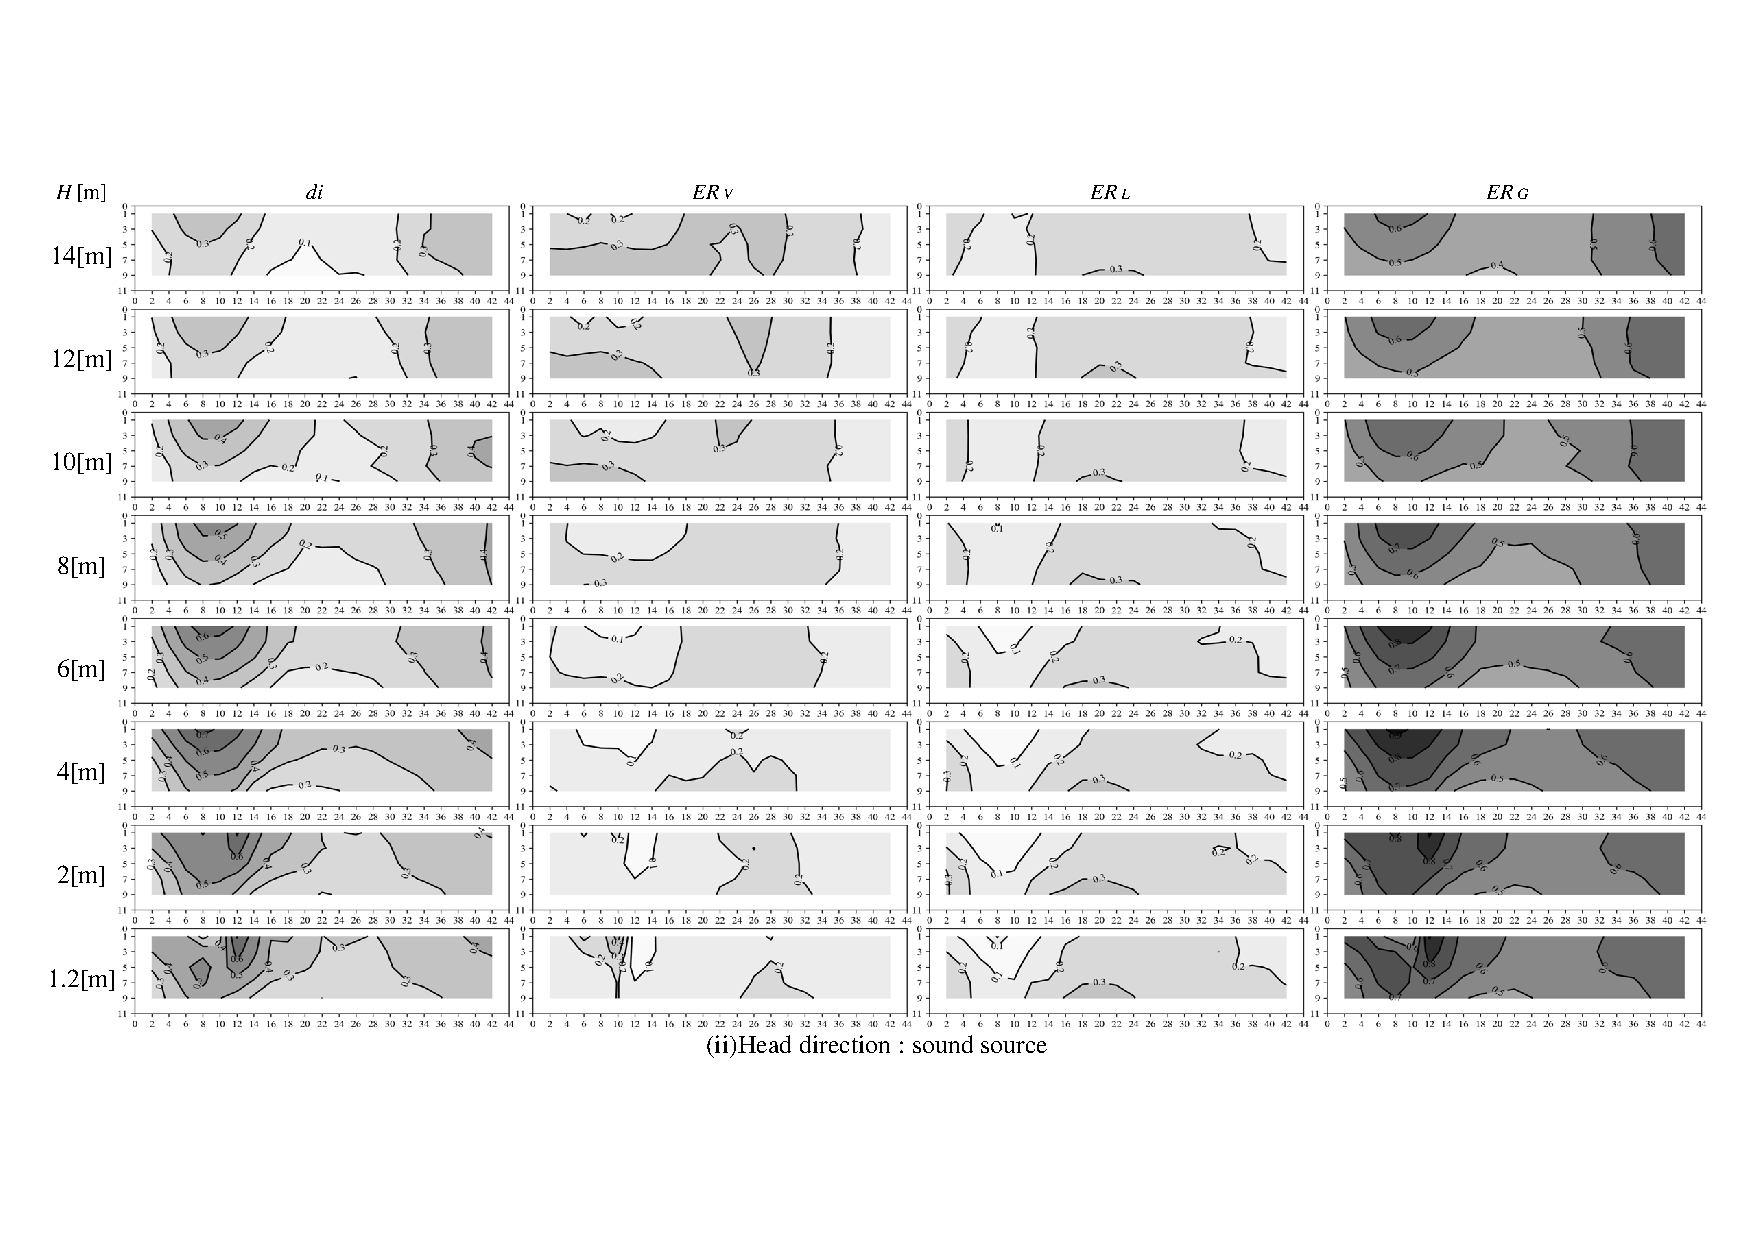
\includepdf[pages=-]{05_att/cont_s.pdf}

\subsubsection{(i)正面:y軸負の方向の場合}
天井付近では天井からの反射音が豊富に到来するが、座席部前方では前後方向成分が多くなり、座席後方では鉛直方向成分が多くなる。
すなわち、観測高さ$H$が高い音場では座席部前方で$ER_V$が、座席部後方で$ER_G$が大きな値をとっている(\figref{er_reason})。
一方、$ER_L$が音源付近で高い値をとっている。これは、頭の方向が常にy軸負の方向を向いているため、両耳方向に音源からの直接音が到来し、側方成分が多くなったと考えられる。
\\
\begin{figure}[htbp]
    \centering
    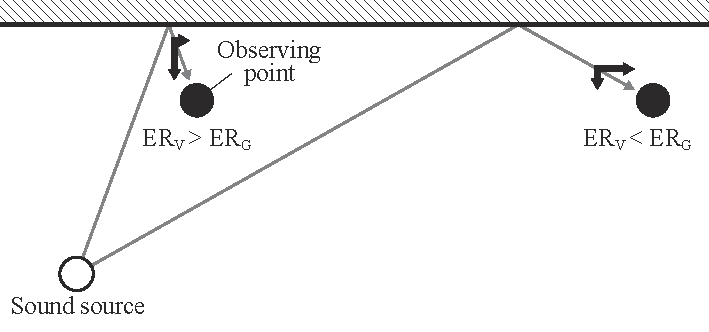
\includegraphics[keepaspectratio,scale=1]{05_att/er_reason.pdf}
    \caption{\hspace{1mm}\textbf{$ER_V$ vs $ER_G$}}
    \label{fig:er_reason}
\end{figure}

\subsubsection{(ii)正面:音源方向の場合}
常に頭が音源を向いているため、直接音は常に前後方向成分に含まれる。$ER_V$、$ER_L$、$ER_G$の和は常に1であるから、$ER_V$と$ER_L$に比べ$ER_G$が全体的に高い値をとっている。側壁付近で$ER_L$が高い値をとっているが、これは頭が音源を向いているため、両耳方向と側壁からの反射音の入射角が合うためであると考えられる。
\\ 本研究では実際にコンサートホールで音を聴いたときに受ける印象と反射音方向分布に符合する(ii)頭の向きを音源としたときの条件で解析を行う。
\pagebreak

\section{観測高さの違いと反射音方向分布特性の分析}


\section{客席面吸音率の変化と反射音方向分布特性の分析}


このとき、$t_A$を最初の反射音が到達するまでの時間、$p_A(t)$を音源からの距離が10mの観測点における直接音の音圧とする。

\begin{equation}
  \label{eq:}
  G_{early} = 10\log_{10}{\frac{\displaystyle\int_0^{80}p^2(t)dt}{\displaystyle\int_0^{t_A}p_{A}^2(t)dt}} \dB
\end{equation}

\begin{equation}
  \label{eq:}
  VG_{early} = 10\log_{10}{\frac{\displaystyle\int_0^{80}p^2(t)cos^2{\delta}dt}{\displaystyle\int_0^{t_A}p_{A}^2(t)dt}} \dB
\end{equation}

\begin{equation}
  \label{eq:}
  LG_{early} = 10\log_{10}{\frac{\displaystyle\int_0^{80}p^2(t)sin^2{\delta}cos^2{\theta}dt}{\displaystyle\int_0^{t_A}p_{A}^2(t)dt}} \dB
\end{equation}

\begin{equation}
  \label{eq:}
  GG_{early} = 10\log_{10}{\frac{\displaystyle\int_0^{80}p^2(t)sin^2{\delta}sin^2{\theta}dt}{\displaystyle\int_0^{t_A}p_{A}^2(t)dt}} \dB
\end{equation}

